\documentclass[11pt,a4paper]{article}
\usepackage{geometry}
\geometry{top=2.5cm, bottom=2.5cm, left=2.5cm, right=2.5cm}
\usepackage{graphicx}
\usepackage{setspace}
\usepackage{tikz}
\usetikzlibrary{calc,positioning,arrows.meta}
\usepackage{eso-pic}
\usepackage{titlesec}
\usepackage{float} % اضافه شدن پکیج float برای ثابت کردن جای عکس‌ها
\titleformat{\section}{\fontsize{18pt}{22pt}\bfseries}{\thesection}{1em}{}
\titleformat{\subsection}{\fontsize{15pt}{19pt}\bfseries}{\thesubsection}{1em}{}

\usepackage{tocloft}
\renewcommand{\cftsecleader}{\cftdotfill{\cftdotsep}}

\usepackage{booktabs}
\usepackage{listings}
\usepackage{xcolor}

\usepackage[pagebackref=false]{hyperref}
\hypersetup{
    colorlinks=true,
    linkcolor=blue,
    citecolor=blue,
    urlcolor=blue
}

\usepackage{xepersian}
\settextfont[
    Path = fonts/ ,
    Extension = .TTF
]{Nilofar_Font}

\setlatintextfont{Times New Roman} 

% ----------------------------------------------------------------
% تنظیمات نمایش کد Verilog در گزارش
% ----------------------------------------------------------------
\lstdefinelanguage{Verilog}{
    morekeywords={module, endmodule, input, output, wire, reg, parameter,
                  localparam, always, posedge, negedge, begin, end, if, else,
                  for, generate, endgenerate, genvar, assign, function,
                  endfunction, integer, initial, task, endtask, case, endcase},
    morecomment=[l]{//},
    morecomment=[s]{/*}{*/},
    morestring=[b]",
    sensitive=true
}
\lstset{
    language=Verilog,
    basicstyle=\ttfamily\footnotesize,
    keywordstyle=\color{blue}\bfseries,
    commentstyle=\color{teal},
    stringstyle=\color{purple},
    numbers=left,
    numberstyle=\tiny\color{gray},
    breaklines=true,
    frame=single,
    backgroundcolor=\color{gray!5},
    tabsize=2,
    showstringspaces=false
}

\begin{document}

\AddToShipoutPictureBG{
    \begin{tikzpicture}[remember picture, overlay]
        \node[draw, line width=2.5pt, minimum width=\paperwidth-2cm, minimum height=\paperheight-2cm, inner sep=0pt] at (current page.center) {};
        \node[draw, line width=1.0pt, minimum width=\paperwidth-2.3cm, minimum height=\paperheight-2.3cm, inner sep=0pt] at (current page.center) {};
    \end{tikzpicture}
}

\begin{titlepage}
    \centering
    \vspace*{0.5cm}
    
\includegraphics[width=3.5cm]{images/logo.png} \\[0.6cm]
    {\fontsize{14pt}{18pt}\selectfont دانشگاه صنعتی شریف} \\[0.2cm]
    {\fontsize{14pt}{18pt}\selectfont دانشکده مهندسی کامپیوتر}

    \vspace{2.5cm}
    {\fontsize{12pt}{16pt}\selectfont عنوان:} \\[0.5cm]
    {\fontsize{22pt}{28pt}\bfseries پیاده‌سازی حافظه شرکت‌پذیر نوع سه‌گانه } \\[0.4cm]

    \vspace{1.5cm}
    {\fontsize{12pt}{16pt}\selectfont نام درس} \\[0.4cm]
    {\fontsize{14pt}{18pt}\bfseries آزمایشگاه طراحی سامانه‌های رقمی }

    \vspace{1.5cm}
    {\fontsize{12pt}{16pt}\selectfont تابستان ۱۴۰۵}

    \vspace{1.5cm}
    {\fontsize{12pt}{16pt}\selectfont دستیار آموزشی} \\[0.4cm]
    {\fontsize{14pt}{18pt}\bfseries علی اثنی‌عشری}

\vspace{1.5cm}
{\fontsize{12pt}{16pt}\selectfont گروه 2\par}
\vspace{0.4cm}
{\fontsize{14pt}{20pt}\bfseries
علی سلطانی - 403106092\\[0.2cm]
یگانه کربلایی - 403106527\\[0.2cm]
محمدمهدی مرادی - 403106681\par}

    \vfill
\end{titlepage}

\newpage
\tableofcontents
\newpage

% ==================================================================
\section{هدف آزمایش}
% ==================================================================
هدف این آزمایش، طراحی و پیاده‌سازی یک پیمانه حافظه شرکت‌پذیر نوع سه‌گانه
\LTRfootnote{Ternary Content Addressable Memory} موسوم به \lr{TCAM} است. این پیمانه
باید شامل ۱۶ ثبات ۱۶ بیتی باشد به‌گونه‌ای که هر بیت از هر ثبات بتواند یکی از
سه مقدار \lr{0}، \lr{1} یا \lr{X} \LTRfootnote{Don't Care} را ذخیره
کند. طراحی باید کاملاً پارامتریک بوده و برای سنتز روی بورد \lr{FPGA} مناسب
باشد. علاوه بر پیاده‌سازی منطق ذخیره‌سازی و مقایسه، صحت عملکرد پیمانه باید
با استفاده از یک فایل آزمون \LTRfootnote{Testbench} در نرم‌افزار \lr{ModelSim}
بررسی شود و گزارش کامل مراحل طراحی، تصمیمات اتخاذشده و نتایج شبیه‌سازی ارائه
گردد.

% ==================================================================
\section{مبانی نظری}
% ==================================================================

حافظه شرکت‌پذیر \LTRfootnote{Content Addressable Memory-CAM} 
برخلاف حافظه‌های معمولی که با آدرس به محتوا دسترسی پیدا می‌کنند، در جهت
عکس عمل می‌کند: یک الگوی جستجو به آن داده می‌شود و پیمانه مشخص می‌کند که
آیا این الگو در میان محتوای ذخیره‌شده وجود دارد یا خیر، و در صورت وجود،
آدرس (یا آدرس‌های) محل آن را برمی‌گرداند. این نوع حافظه به‌طور گسترده در
کاربردهایی مانند جدول مسیریابی شبکه، حافظه‌های نهان \LTRfootnote{Cache}، فشرده‌سازی
داده، بانک داده و سامانه‌های هوشمند به کار می‌رود.

حافظه شرکت‌پذیر نوع سه‌گانه \LTRfootnote{Ternary}
تعمیمی از \lr{CAM} معمولی است. تفاوت اصلی آن با \lr{CAM} عادی این است که
علاوه بر مقادیر \lr{0} و \lr{1}، هر بیت از هر ثبات می‌تواند مقدار \lr{X} نیز داشته باشد. به این معنا که در فرایند مقایسه وانطباق \LTRfootnote{Match}،
بیت‌های \lr{X} نادیده گرفته می‌شوند و صرف‌نظر از مقدار بیت متناظر در الگوی
جستجو، همواره با آن منطبق در نظر گرفته می‌شوند. برای مثال، اگر داده
\lr{01101110} در یک \lr{TCAM} جستجو شود، با هر یک از الگوهای زیر که در
ثبات‌های آن ذخیره شده باشند به عنوان انطباق شناسایی می‌شود:
\begin{center}
\lr{0110XXXX} \quad \lr{X1101XXX} \quad \lr{0X1X11X0} \quad \lr{XXXXXXXX}
\end{center}
این ویژگی، \lr{TCAM} را برای کاربردهایی مانند طبقه‌بندی بسته‌های شبکه و
جدول‌های مسیریابی با پیشوند متغیر \LTRfootnote{Longest Prefix Match} بسیار مناسب
می‌کند، چرا که یک قانون واحد می‌تواند به‌طور هم‌زمان بازه‌ای از آدرس‌ها را
پوشش دهد.

% ==================================================================
\section{طراحی و الگوریتم پیاده‌سازی}
% ==================================================================

\subsection{نمایش داده سه‌مقداری}
از آنجا که سخت‌افزارهای رقمی معمولی تنها دو حالت \lr{0} و \lr{1} را
پشتیبانی می‌کنند، برای نمایش حالت سوم (\lr{X}) از یک نمایش دوکلمه‌ای استفاده
شده است. برای هر ثبات، دو کلمه ۱۶ بیتی نگهداری می‌شود:
\begin{itemize}
    \item \lr{\texttt{data}}: مقدار \lr{0} یا \lr{1} هر بیت را نگه می‌دارد.
    \item \lr{\texttt{mask}}: تعیین می‌کند که آیا آن بیت باید در مقایسه
          شرکت داده شود (\lr{1}) یا فاقد اهمیت\LTRfootnote{Don't Care} است (\lr{0}).
\end{itemize}
با این نمایش، رابطه انطباق برای بیت $j$ اُم از ثبات $i$ اُم به‌صورت زیر
تعریف می‌شود:
\[
    \mathrm{term}_i(j) \;=\; \overline{\mathrm{mask}_i(j)} \;\lor\; \overline{\mathrm{data}_i(j) \oplus \mathrm{search}(j)}
\]
یعنی اگر آن بیت  باشد ($\mathrm{mask}_i(j)=0$)، عبارت همواره
درست است؛ در غیر این صورت باید بیت داده دقیقاً با بیت الگوی جستجو برابر
باشد. برای این‌که ثبات $i$ اُم به‌طور کامل با الگوی جستجو منطبق شناخته
شود، باید تمام ۱۶ بیت آن شرط را برآورده کنند:
\[
    \mathrm{match}_i \;=\; \bigwedge_{j=0}^{15} \mathrm{term}_i(j)
\]

\subsection{بیت اعتبار \lr{(Valid)}}
یکی از نکات ظریفی که در حین طراحی و شبیه‌سازی مشخص شد، رفتار ثبات‌های
هنوز برنامه‌ریزی‌نشده است. اگر پس از ریست، کلمه \lr{\texttt{mask}} تمام
ثبات‌ها صفر باشد، این به معنای آن است که تمام بیت‌های آن‌ها \lr{Don't Care}
هستند؛ در نتیجه چنین ثباتی با \emph{هر} الگوی جستجویی منطبق می‌شود که
کاملاً نادرست و گمراه‌کننده است. برای رفع این مشکل، یک بیت مستقل به نام
\lr{\texttt{valid}} برای هر ثبات اضافه شد که تنها پس از نوشتن واقعی در آن
آدرس به مقدار یک تنظیم می‌شود. رابطه نهایی انطباق به‌صورت زیر اصلاح شد:
\[
    \mathrm{match}_i \;=\; \mathrm{valid}_i \;\land\; \bigwedge_{j=0}^{15} \mathrm{term}_i(j)
\]
این تغییر با شبیه‌سازی نیز تأیید شد: در سناریوی آزمون شماره ۵ (بخش
\ref{sec:sim})، یک الگوی کاملاً تصادفی جستجو شد و مشاهده شد که تنها ثبات
از پیش برنامه‌ریزی‌شده (ثبات ۳ که کاملاً \lr{Don't Care} تعریف شده بود) با آن منطبق
می‌شود، نه ثبات‌های نانوشته ۴ تا ۱۵.

\subsection{نمودار بلوکی پیمانه}
شکل \ref{fig:block} نمای کلی ورودی‌ها و خروجی‌های پیمانه \lr{TCAM} طراحی‌شده
را نشان می‌دهد.

\begin{figure}[H]
\centering
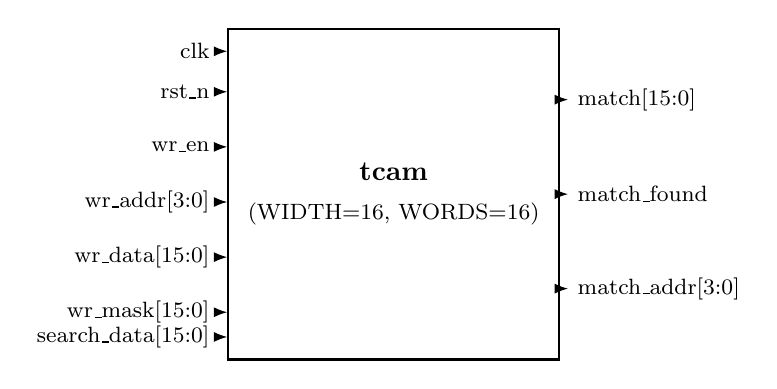
\begin{tikzpicture}[
    block/.style={draw, minimum width=4.2cm, minimum height=4.2cm, thick},
    port/.style={font=\footnotesize}
]
\node[block, align=center] (tcam) {\lr{\bfseries tcam}\\[2pt]{\footnotesize\lr{(WIDTH=16, WORDS=16)}}};

% ورودی‌ها (سمت چپ)
\node[port, left=0.1cm of tcam.north west, anchor=east, yshift=-0.3cm] (clk) {\lr{clk}};
\node[port, left=0.1cm of tcam.west, anchor=east, yshift=1.3cm] (rst) {\lr{rst\_n}};
\node[port, left=0.1cm of tcam.west, anchor=east, yshift=0.6cm] (wren) {\lr{wr\_en}};
\node[port, left=0.1cm of tcam.west, anchor=east, yshift=-0.1cm] (wraddr) {\lr{wr\_addr[3:0]}};
\node[port, left=0.1cm of tcam.west, anchor=east, yshift=-0.8cm] (wrdata) {\lr{wr\_data[15:0]}};
\node[port, left=0.1cm of tcam.west, anchor=east, yshift=-1.5cm] (wrmask) {\lr{wr\_mask[15:0]}};
\node[port, left=0.1cm of tcam.south west, anchor=east, yshift=0.3cm] (search) {\lr{search\_data[15:0]}};

\draw[-{Latex}] (clk.east) -- ([yshift=-0.3cm]tcam.north west);
\draw[-{Latex}] (rst.east) -- ([yshift=1.3cm]tcam.west);
\draw[-{Latex}] (wren.east) -- ([yshift=0.6cm]tcam.west);
\draw[-{Latex}] (wraddr.east) -- ([yshift=-0.1cm]tcam.west);
\draw[-{Latex}] (wrdata.east) -- ([yshift=-0.8cm]tcam.west);
\draw[-{Latex}] (wrmask.east) -- ([yshift=-1.5cm]tcam.west);
\draw[-{Latex}] (search.east) -- ([yshift=0.3cm]tcam.south west);

% خروجی‌ها (سمت راست)
\node[port, right=0.1cm of tcam.east, anchor=west, yshift=1.2cm] (match) {\lr{match[15:0]}};
\node[port, right=0.1cm of tcam.east, anchor=west, yshift=0cm] (found) {\lr{match\_found}};
\node[port, right=0.1cm of tcam.east, anchor=west, yshift=-1.2cm] (maddr) {\lr{match\_addr[3:0]}};

\draw[-{Latex}] ([yshift=1.2cm]tcam.east) -- (match.west);
\draw[-{Latex}] ([yshift=0cm]tcam.east) -- (found.west);
\draw[-{Latex}] ([yshift=-1.2cm]tcam.east) -- (maddr.west);
\end{tikzpicture}
\caption{نمودار بلوکی پیمانه \lr{tcam} همراه با پورت‌های ورودی و خروجی}
\label{fig:block}
\end{figure}

\subsection{منطق نوشتن (برنامه‌ریزی ثبات‌ها)}
نوشتن در پیمانه به‌صورت همزمان \LTRfootnote{Synchronous} و روی لبه بالارونده
ساعت\LTRfootnote{Clock} انجام می‌شود. با فعال بودن سیگنال \lr{\texttt{wr\_en}}، مقادیر
\lr{\texttt{wr\_data}} و \lr{\texttt{wr\_mask}} در آدرس \lr{\texttt{wr\_addr}}
نوشته شده و بیت \lr{\texttt{valid}} متناظر یک می‌شود. با فعال شدن سیگنال
ریست (\lr{\texttt{rst\_n}}) با مقدار پایین، تمام ثبات‌ها به حالت نامعتبر
بازمی‌گردند.

\subsection{منطق مقایسه و انکودر اولویت}
منطق مقایسه به‌صورت کاملاً ترکیبی \LTRfootnote{Combinational} و با استفاده از
حلقه \lr{\texttt{generate}} برای هر ۱۶ ثبات پیاده‌سازی شده است؛ به این
ترتیب طراحی نسبت به پارامترهای \lr{\texttt{WIDTH}} و \lr{\texttt{WORDS}}
به‌طور کامل مقیاس‌پذیر است. در صورتی که بیش از یک ثبات با الگوی جستجو
منطبق شود (که در \lr{TCAM} کاملاً محتمل و بخشی از کاربرد آن است)، خروجی
\lr{\texttt{match\_addr}} با استفاده از یک تابع انکودر اولویت، آدرس اولین
ثبات (کمترین زیروند) منطبق را گزارش می‌کند. خروجی \lr{\texttt{match\_found}}
نیز به‌سادگی \lr{OR} منطقی تمام بیت‌های بردار \lr{\texttt{match}} است.

% ==================================================================
\section{پیاده‌سازی \lr{Verilog}}
% ==================================================================
پیمانه به‌طور کامل با زبان \lr{Verilog} و به‌صورت پارامتریک (با پارامترهای
\lr{\texttt{WIDTH}} و \lr{\texttt{WORDS}}) نوشته شده است. فایل کامل 
 طراحی (\lr{\texttt{tcam.v}}) و فایل آزمون
(\lr{\texttt{tcam\_tb.v}}) به‌طور کامل همراه این گزارش ارسال شده‌اند. در
ادامه، هسته اصلی منطق مقایسه و انکودر اولویت  (که مهم‌ترین بخش الگوریتمی
طراحی است)  آورده شده است:

\begin{latin}
\begin{lstlisting}[caption={Core match logic and priority encoder (excerpt from tcam.v)}]
genvar g;
generate
    for (g = 0; g < WORDS; g = g + 1) begin : gen_match
        assign match[g] = valid_mem[g] &
             ( &( ~mask_mem[g] | ~(data_mem[g] ^ search_data) ) );
    end
endgenerate

assign match_found = |match;

function [ADDR_W-1:0] priority_encode;
    input [WORDS-1:0] m;
    integer k;
    begin
        priority_encode = {ADDR_W{1'b0}};
        for (k = WORDS-1; k >= 0; k = k - 1)
            if (m[k]) priority_encode = k[ADDR_W-1:0];
    end
endfunction

assign match_addr = priority_encode(match);
\end{lstlisting}
\end{latin}

\subsection{پارامتریک بودن طراحی}
پارامترهای \lr{\texttt{WIDTH}} (عرض هر ثبات، مقدار پیش‌فرض ۱۶) و
\lr{\texttt{WORDS}} (تعداد ثبات‌ها، مقدار پیش‌فرض ۱۶) در ابتدای پیمانه
تعریف شده‌اند و عرض باس آدرس (\lr{\texttt{ADDR\_W}}) نیز به‌طور خودکار با
استفاده از تابع \lr{\texttt{\$clog2}} از روی \lr{\texttt{WORDS}} محاسبه
می‌شود. به این ترتیب، برای تغییر ابعاد پیمانه (مثلاً به ۳۲ ثبات ۳۲ بیتی)
تنها کافی است مقدار این دو پارامتر در نمونه‌سازی پیمانه تغییر کند و نیازی
به تغییر کد داخلی نیست.

% ==================================================================
\section{شبیه‌سازی و تست}
\label{sec:sim}
% ==================================================================

\subsection{سناریوهای آزمون}
برای اطمینان از صحت عملکرد پیمانه، یک فایل آزمون در \lr{ModelSim} نوشته
شد که پنج سناریوی زیر را پوشش می‌دهد. ابتدا چهار ثبات با ماسک‌های متفاوت
برنامه‌ریزی می‌شوند (جدول \ref{tab:program})، سپس پنج الگوی جستجو اعمال
می‌شود (جدول \ref{tab:results}):

\begin{table}[H]
\centering
\caption{ثبات‌های برنامه‌ریزی‌شده در فایل آزمون}
\label{tab:program}
\begin{tabular}{ccll}
\toprule
آدرس & \lr{data} & \lr{mask} & توضیح \\
\midrule
0 & \lr{0x006E} & \lr{0x00FF} & الگوی کاملاً مشخص \lr{(0110\_1110)}، بدون \lr{X} \\
1 & \lr{0x0060} & \lr{0x00F0} & الگوی \lr{0110XXXX} (نیمه پایین \lr{X}) \\
2 & \lr{0x000E} & \lr{0x000F} & الگوی \lr{XXXX1110} (نیمه بالا \lr{X}) \\
3 & \lr{0x0000} & \lr{0x0000} & کاملاً \lr{X} \lr{---} با هر مقداری منطبق می‌شود \\
\bottomrule
\end{tabular}
\end{table}

\begin{table}[H]
\centering
\caption{نتایج پنج سناریوی جستجو (خروجی تأییدشده در شبیه‌سازی)}
\label{tab:results}
\begin{tabular}{clcc}
\toprule
تست & الگوی جستجو \lr{(search\_data)} & \lr{match} (باینری) & \lr{match\_addr} \\
\midrule
۱ & \lr{0x006E} \lr{---} تطابق دقیق با ثبات ۰ & \lr{0000000000001111} & ۰ \\
۲ & \lr{0x0065} \lr{---} تست نیمه پایین \lr{X} & \lr{0000000000001010} & ۱ \\
۳ & \lr{0x000E} \lr{---} تست نیمه بالا \lr{X} & \lr{0000000000001100} & ۲ \\
۴ & \lr{0x00FF} \lr{---} فقط باید با ثبات کاملاً \lr{X} منطبق شود & \lr{0000000000001000} & ۳ \\
۵ & \lr{0xABCD} \lr{---} الگوی کاملاً تصادفی (بررسی ثبات‌های نانوشته) & \lr{0000000000001000} & ۳ \\
\bottomrule
\end{tabular}
\end{table}

نکته مهم در تست شماره ۵: با وجود آنکه الگوی جستجو کاملاً دلخواه و
بی‌ارتباط با محتوای برنامه‌ریزی‌شده است، بردار \lr{match} تنها بیت مربوط به
ثبات ۳ (که عمداً کاملاً دون‌کر تعریف شده) را یک نشان می‌دهد و بیت‌های
مربوط به ثبات‌های ۴ تا ۱۵ (که هرگز نوشته نشده‌اند) صفر باقی می‌مانند. این
دقیقاً همان رفتاری است که با افزودن بیت \lr{valid} انتظار می‌رفت و صحت این
تصمیم طراحی را تأیید می‌کند.

\subsection{نتیجه موج شبیه‌سازی}
شکل \ref{fig:wave} خروجی پنجره موج \lr{ModelSim} پس از اجرای کامل فایل
آزمون را نشان می‌دهد. در بازه ابتدایی (تا نانوثانیه ۴۰ام) چهار عملیات
نوشتن روی ثبات‌های ۰ تا ۳ قابل مشاهده است (تغییرات \lr{wr\_addr}،
\lr{wr\_data} و \lr{wr\_mask}) و در ادامه، برای هر یک از پنج الگوی جستجو،
تغییر متناظر در \lr{match}، \lr{match\_found} و \lr{match\_addr} دیده
می‌شود که کاملاً با مقادیر جدول \ref{tab:results} مطابقت دارد.

\begin{figure}[H]
\centering
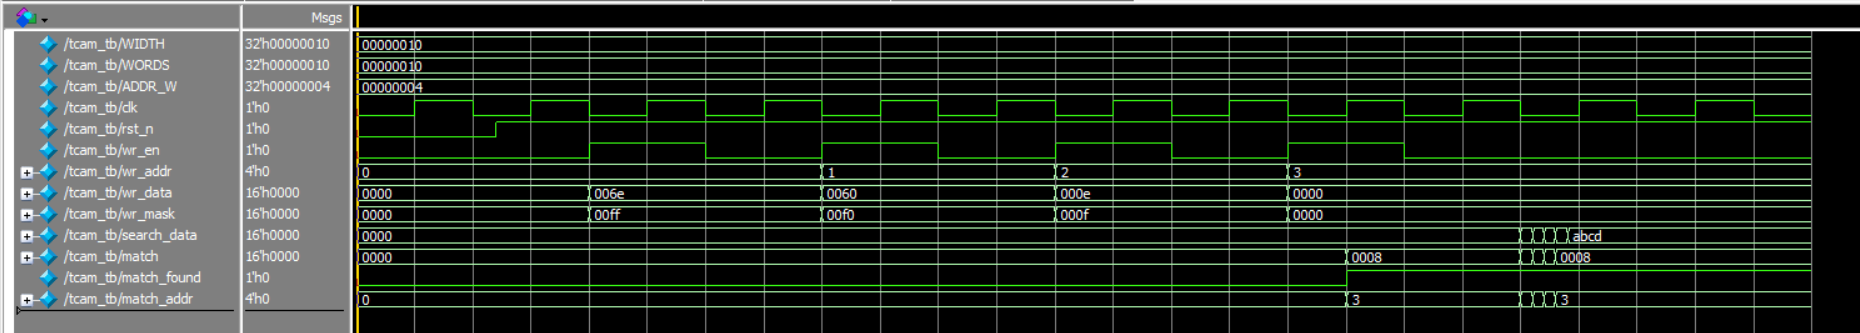
\includegraphics[width=\textwidth]{images/modelsim_wave.png}
\caption{پنجره موج \lr{ModelSim} پس از اجرای فایل آزمون \lr{---} عملیات نوشتن
چهار ثبات و نتیجه پنج جستجو}
\label{fig:wave}
\end{figure}

% ==================================================================
\section{سنتز و بررسی منابع مصرفی روی \lr{FPGA}}
% ==================================================================
پس از تأیید صحت عملکرد در شبیه‌سازی، طراحی در نرم‌افزار \lr{Quartus} با
پیمانه \lr{\texttt{tcam}} به‌عنوان \lr{Top-Level Entity} سنتز شد. خلاصه
مصرف منابع گزارش‌شده توسط \lr{Analysis \& Synthesis} در جدول
\ref{tab:resources} آمده است.

\begin{table}[H]
\centering
\caption{خلاصه مصرف منابع منطقی پس از سنتز (\lr{Analysis \& Synthesis Summary})}
\label{tab:resources}
\begin{tabular}{lc}
\toprule
پارامتر & مقدار \\
\midrule
تعداد عناصر منطقی  & \lr{879} (\lr{351 Combinational}) \\
تعداد ثبات‌ها  & \lr{528} \\
حداکثر بسامد کاری تخمینی  & \lr{N/A} \\
\bottomrule
\end{tabular}
\end{table}

\begin{figure}[H]
\centering
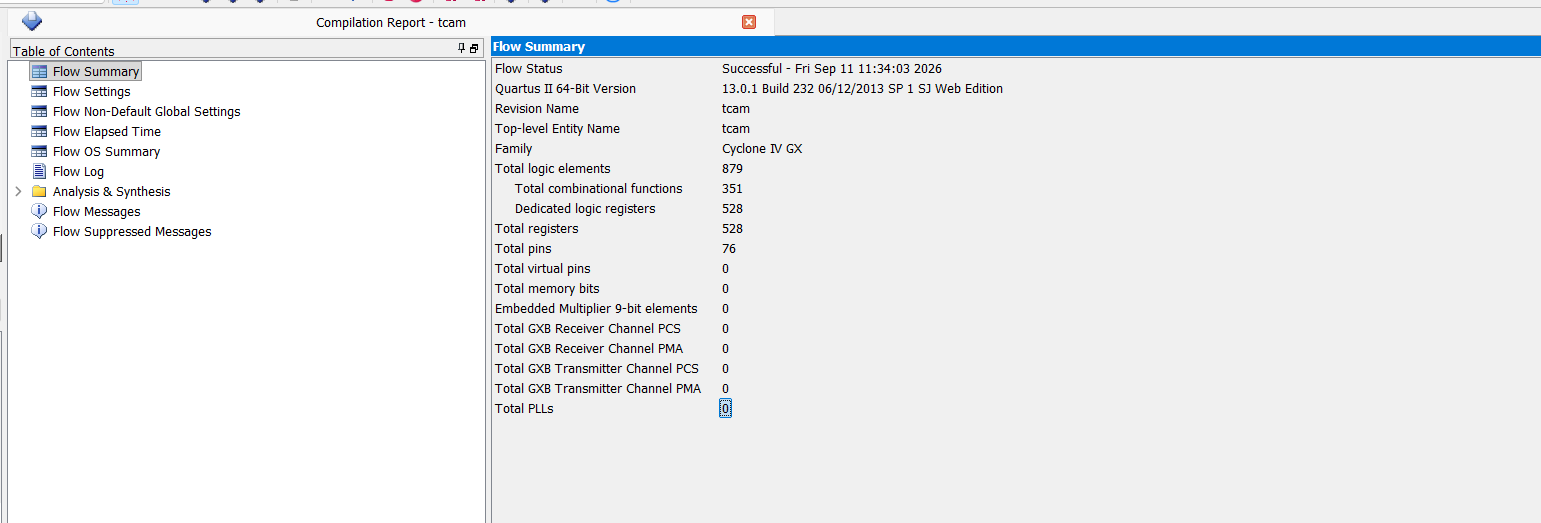
\includegraphics[width=0.85\textwidth]{images/quartus_synthesis_summary.png}
\caption{خلاصه گزارش سنتز در \lr{Quartus}}
\label{fig:synth}
\end{figure}

از آنجا که طراحی برای ابعاد ۱۶ ثبات ۱۶ بیتی ($16\times16=256$ سلول
سه‌مقداری) پیاده‌سازی شده، مصرف منابع منطقی (\lr{LUT} و ثبات) در حد معقولی
باقی می‌ماند و مشکلی برای سنتز روی بورد آموزشی ایجاد نمی‌کند. لازم به ذکر
است که این پیاده‌سازی کاملاً مبتنی بر ثبات و منطق ترکیبی
(\lr{Register + LUT based}) است، در حالی‌که پیاده‌سازی‌های صنعتی واقعی
\lr{TCAM} معمولاً از حافظه‌های \lr{BRAM} یا سلول‌های حافظه اختصاصی سه‌مقداری
استفاده می‌کنند تا در ابعاد بزرگ (هزاران ورودی) از مصرف بیش از حد منابع
\lr{LUT} جلوگیری شود. برای ابعاد کوچک این آزمایش، رویکرد مبتنی بر منطق
ترکیبی انتخاب مناسب و کافی است.

% ==================================================================
\section{ملاحظات پیاده‌سازی روی بورد \lr{FPGA}}
% ==================================================================
یکی از محدودیت‌های عملی پیاده‌سازی این طرح روی بورد \lr{FPGA}، تعداد
ورودی‌های مورد نیاز است. برای بهره‌گیری کامل از پیمانه، باید بتوان
\lr{\texttt{wr\_addr}} (۴ بیت)، \lr{\texttt{wr\_data}} (۱۶ بیت)،
\lr{\texttt{wr\_mask}} (۱۶ بیت) و \lr{\texttt{search\_data}} (۱۶ بیت) را
از طریق سوییچ‌های فیزیکی بورد وارد کرد که مجموعاً ۵۲ بیت است. 

برای رفع این محدودیت، ورودی به‌صورت \textbf{مرحله‌ای} وارد
خواهد شد: با استفاده از چند سوییچ برای انتخاب حالت (نوشتن آدرس، نوشتن
داده، نوشتن ماسک یا جستجو) و یک ثبات شیفت داخلی که با فشردن یک دکمه،
مقادیر سوییچ‌های ورودی را به‌تدریج در یک ثبات میانی بارگذاری می‌کند، امکان
وارد کردن مقادیر چندبیتی با تعداد محدودی سوییچ فراهم می‌شود. خروجی
\lr{\texttt{match}}، \lr{\texttt{match\_found}} و \lr{\texttt{match\_addr}}
نیز با توجه به تعداد \lr{LED} و نمایشگر هفت‌قسمتی موجود روی بورد، به‌صورت
چندمرحله‌ای یا با کدگذاری \lr{Hex} روی نمایشگر نمایش داده خواهد شد.

% ==================================================================
\section{نتیجه‌گیری}
% ==================================================================
در این آزمایش، یک پیمانه حافظه شرکت‌پذیر سه‌گانه \LTRfootnote{TCAM} با ۱۶ ثبات
۱۶ بیتی و به‌صورت کاملاً پارامتریک طراحی و پیاده‌سازی شد. نمایش سه‌مقداری
هر بیت با استفاده از دو کلمه \lr{data} و \lr{mask} انجام شد و برای رفع
مشکل انطباق نادرست ثبات‌های نانوشته، بیت اعتبار \LTRfootnote{valid} به طراحی
اضافه گردید. تصمیمی که با شبیه‌سازی مورد تأیید قرار گرفت. عملکرد طرح با
پنج سناریوی آزمون مختلف در \lr{ModelSim} بررسی و صحت کامل آن (شامل تطابق
دقیق، تطابق با بیت‌های \lr{X} در نیمه‌های مختلف کلمه، و رفتار صحیح ثبات‌های
نانوشته) تأیید شد. طراحی سپس در \lr{Quartus} با موفقیت سنتز شد. در نهایت،
محدودیت تعداد ورودی‌های فیزیکی بورد در برابر عرض ۱۶ بیتی داده‌ها بررسی و
راهکار ورودی مرحله‌ای برای پیاده‌سازی عملی روی بورد پیشنهاد شد.

\end{document}
